\simpleheading{Introduction}

The project uses text data on day-to-day legislative activity to map together bills, motions, questions, speeches, and votes. The project also includes data on members, constituencies, and committees, among other things. The project covers XX parliaments: the XX Parliament (starting XX XX, 2XXX) through most of the XX Parliament (through XX XX, 2019). %This includes eight parliamentary sessions (39-1, 39-2, 40-1, 40-2, 40-3, 41-1, 41-2, and 42-1).

Sources of data include \highlight{Hansard} (legislative minutes), the \highlight{Order Paper}, and \href{https://commonsvotes.digiminster.com/}{\highlight{CommonsVotes}} (Parliament's official database of bills and votes). These sources are discussed in detail below.

\myline

\subheading{Legislative Process}

This project tracks the progression of bills through the legislative process and connects them with other legislative activity, including questions, speeches, and votes. The legislative process consists of the following steps, which are also outlined in Figure~\ref{fig:legislativeProcess}:

\begin{itemize}

	\item \highlight{The introduction and first reading of a bill:} Though largely a formaility, the short title of bills are read aloud and they are ordered to be "printed" in the official journal. This indicates that the bill can proceed to the next stage, which will be the first opportunity for MPs to debate the bill's general principles and themes.

	\item \highlight{The second reading and referral to a committee:} The Government minister, spokesperson or MP responsible for the bill begins the debate and the official Opposition spokesperson responds. The debate continues with other Opposition parties and backbenchers giving their opinions. At the end of the debate, the House of Commons as a whole decides whether the bill should be given its second reading by voting so it can proceed to the next stage. It is possible for a bill to have a second reading with no debate, as long as MPs agree. The second reading usually takes place no sooner than two weekends after first reading.

	\item \highlight{The committee stage:} The committee reviews the text of the bill and each clause or amendments may be debated. Every clause in the bill is agreed to, although this may happen (particularly under a programme order) without debate.	Amendments for discussion are selected by the committee chairman and only committee members can vote on amendments. Amendments proposed by MPs to the bill are then published daily, so if the bill is amended it will be reprinted before its next stage. Once committee stage is finished, the bill returns to the floor for further debate and amendment proposals.
	
	%When the bill originates in the House of Commons, the committee is able to take evidence from experts and interest groups from outside Parliament.
	%Amendments proposed by MPs to the bill are then published daily and reprinted each day the committee discusses that particular bill. Most bills pass through a "Public Bill Committee". 	
	%Consolidated Fund Bills do not have a committee stage at all.
	%A minority of Bills are dealt with by a Committee of the whole House (takes place on the floor of the House of Commons), with every MP able to take part. The selection and grouping of amendments in a Committee of the whole House is decided by the Chairman of Ways and Means (Deputy Speaker).
	%Bills fast tracked through the House of Commons will receive less consideration.  
	
	\item \highlight{The report stage:} During this stage, members can propose motions to amend the bill (called report stage motions). These motions appear in the \highlight{Report Stage of Bills} section of the Notice Paper. (See the section on the Notice Paper below.) These must be notified 48 hours in advance. Debate is on individual motion to amend the bill, not the bill as a whole. The Speaker can select and group amendments for debate to avoid a repeat of the committee stage. There is only debate at the report stage if there are motions to amend the bill.
	\item \highlight{The third reading and passage:} During this stage, members vote on the bill as a whole. A motion for a third reading and passage can be amended. A motion for a third reading can be amended. Possible amendments include hoist amendments, reasoned amendments, and amendments to recommit the bill to a committee. If the motion for a third reading passes, the bill is considered adopted by the House and is sent to the Senate for consideration.
	\item \highlight{Consideration and passage by the Senate:} During this stage, the Senate debates the bill and can vote on amendments. The House votes on any approved Senate amendments. The House and the Senate can exchange messages to resolve disagreements. The House and the Senate must both approve the same version of the bill.
	\item \highlight{Royal Asset and coming into force:} If the same version of a bill is passed by both the House and the Senate, it is granted Royal Assent by the Governor General and enters into force on the stated date.
\end{itemize}

\begin{figure}[htbp!]
	\caption{\footnotesize{Bill initiation and stages of completion in both upper and lower British chambers.}}
	\label{fig:legislativeProcess}
	\centering
	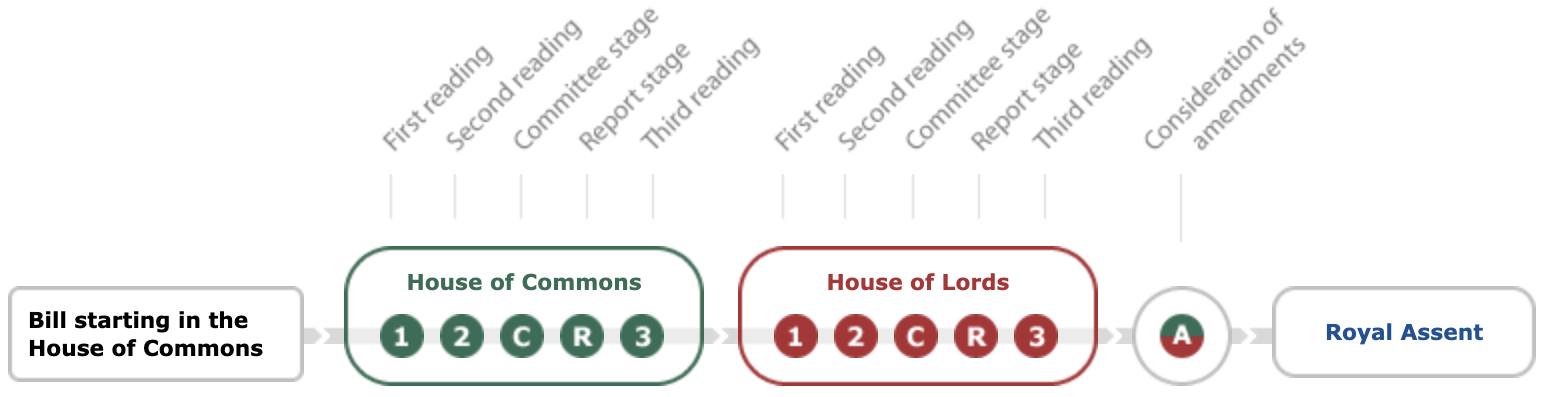
\includegraphics[width=\textwidth]{legislativeProcess.png}\\
	\vspace{.5cm}
	\raggedright   \footnotesize{\textbf{Source:} \href{https://www.parliament.uk/about/how/laws/passage-bill/}{www.parliament.uk}.}
\end{figure}


\myline

\subheading{Order Paper}

%The \highlight{Order Paper} the daily agenda of the House of Commons. It is published every sitting day. It lists all items of business that the House can consider that day. The \highlight{Order Paper} is available online at \code{URL}. The unanimous consent of all members is required to consider items of business that are not listed on the \highlight{Order Paper}. Items on the \highlight{Notice Paper} move to the \highlight{Order Paper} after the notice period is over. The \highlight{Order Paper} is organized into the following sections:
%\begin{itemize}
%	\item \highlight{Order of Business.}
%	\begin{itemize}
%		\item \highlight{Daily Routine of Business.} (Also called Routine Proceedings.)
%		\begin{itemize}
%			\item \highlight{Tabling of Documents.} No notice is required for tabling a document, so this section is always empty.
%			\item \highlight{Introduction of Government Bills.}
%			\item \highlight{Statements by Members.} No notice required for statements by members, so this section is always empty.
%			\item \highlight{Presenting Reports from Interparliamentary Delegations.} No notice required for presenting reports, so this section is always empty.
%			\item \highlight{Presenting Reports from Committees.} No notice required for presenting reports, so this section is always empty.
%			\item \highlight{Introduction of Private Members' Bills.}
%			\item \highlight{First Reading of Senate Public Bills.}
%			\item \highlight{Motions.}
%			\item \highlight{Presenting Petitions.} No notice required is required for presenting petitions, so this section is always empty.
%			\item \highlight{Questions on the Order Paper.} Questions are available online in a separate section at the end of the Order Paper.
%		\end{itemize}
%	\end{itemize}
%	\item \highlight{Orders of the Day.}
%	\begin{itemize}
%		\item \highlight{Government Orders.}
%		\begin{itemize}
%			\item \highlight{Business of Supply.} All opposition motions and motions to concur in interim supply, the main estimates, or supplementary estimates. 
%			\item \highlight{Ways and Means.} All motions related to bills for the raising of revenue.
%			\item \highlight{Government Bills (Commons).} Any bills introduced in the Commons that have had a first reading and are not in committee. This includes bills that are waiting for the second reading stage, report stage, or third reading stage.
%			\item \highlight{Government Bills (Senate).} Any bills sent to the Commons by the Senate that have had a first reading and are not in committee.
%			\item \highlight{Government Business.} Any other government business.
%		\end{itemize}
%		\item \highlight{Concurrence in Committee Reports}
%	\end{itemize}
%	%\item Notices of Motions for the Production of Papers (?)
%	\item \highlight{Private Members' Business.}
%	\begin{itemize}
%		%\item Rescheduled Business (?)
%		%\item Deferred Recorded Divisions (?)
%		\item \highlight{Items in the Order of Precedence.} The first 30 members on the List of the Consideration of Private Members' Business who have introduced a bill or have given notice of a motion. The Standing Orders include rules for changing the order of items, adding items, and dropping items. 
%		\item \highlight{Items outside the Order of Precedence.}
%		\begin{itemize}
%			\item \highlight{Public Bills (Commons).} Public bills that originated in the Commons and that have had a first reading.
%			\item \highlight{Notices of Motions.} Notices of motions that have already been notified.
%			\item \highlight{Notices of Motions (Papers).} Notices of Motions for the Production of Papers that have already been notified.
%		\end{itemize}
%		\item \highlight{List for the Consideration of Private Members' Business.} A list of members that indicates the order in which their business can be considered by the Commons. When there are fewer than 15 names on the list, a new list is created. 
%		\begin{itemize}
%			\item \highlight{Eligible Members.} A list of members who are eligible to have business considered (see Standing Order 87).
%			\item \highlight{Ineligible Members.} A list of members who are not eligible to have business considered (see Standing Order 87). 
%		\end{itemize}
%	\end{itemize}
%	%\item Private Members' Business
%	%\item Private Members' Business (Items outside the Order of Precedence)
%	%\item Private Members' Business (List for the Consideration of Private Members' Business)
%	\item \highlight{Questions.} Online only. A complete list of all notified written questions that have not been answered, withdrawn, or made into orders for return. 
%\end{itemize}
%
%\myline
%
%\subheading{Notice Paper}
%
%The \highlight{Notice Paper} is also published every sitting day. It lists all items that are being notified that day. Most items have to be notified at 48 hours in advance for the House to be able to consider them. After the notification period, items on the \highlight{Notice Paper} are transferred to the \highlight{Order Paper}. The \highlight{Notice Paper} is organized into the following sections: 
%\begin{itemize}
%	\item \highlight{Introduction of Government Bills.} Government bills that are being notified.
%	\item \highlight{Introduction of Private Members' Bills.} Private member bills that are being notified.
%	\item \highlight{Notices of Motions (Routine Proceedings).} Notices of motions.
%	\item \highlight{Questions.} Notices of written questions.
%	\item \highlight{Notices of Motions for the Production of Papers.} Notices of motions for the production of papers.
%	\item \highlight{Business of Supply.} Notices of supply motions and opposition motions.
%	\item \highlight{Government Business.} Notices of motions dealing with government business.
%	\item \highlight{Private Members' Notices of Motions.} Notices of Private Members' Motions.
%	\item \highlight{Private Members' Business.} Notices of Private Members' Bills.
%	\item \highlight{Report Stage of Bills.} 
%	\begin{itemize}
%		\item \highlight{Notices of Motions.} Notices of report stage motions.
%		\item \highlight{Resuming Debate.} A list of report stage motions that are being debated and that have already been notified.
%		\item \highlight{Deferred Recorded Divisions.} A list of deferred recorded divisions that are scheduled to be held.
%	\end{itemize}
%	% \item Motions Respecting Senate Amendments to Bills
%\end{itemize}
%
%\myline
%
%\subheading{Status of House Business}
%
%The \highlight{Status of House Business} is a summary of all items that have appeared on the \highlight{Order Paper} or the \highlight{Notice Paper} over a session. It is published at the end of each session. The \highlight{Status of House Business} is organized into the following sections:
%\begin{itemize}
%	\item \highlight{Part I --- Government Orders}. A summary of the legislative history of government bills and government motions, including supply motions and ways and means motions. Bill entires include the dates that the bill was considered. Motion entries include the subject matter, the date of notice, the dates that the motion was considered, the disposition, and the sponsor. 
%	\item \highlight{Part II --- Private Members' Business}. A summary of all activity related to public bills sponsored by private members, private bills, Private Members' motions, and motions for the production for papers.
%	\item \highlight{Part III --- Written Questions}. A summary of all activity related to written questions. This includes when a question is notified, answered during debate, made an order for return (i.e., in which case the answer will be tabled as a session paper instead of the question being answered during debate), withdrawn, or transferred to the Adjournment Proceedings for debate. 
%	\item \highlight{Part IV --- Business Respecting Committees}. A summary of motions for concurrence in committee reports and other motions related to committees. 
%	\item \highlight{Part V --- Other Business}. A summary of other motions.
%\end{itemize}
%
%\myline
%
%%--------------------------------------------------%
%% datasets
%%--------------------------------------------------%

\newpage

\subheading{Overview of Datasets}

The project includes XX datasets organized into X sectors. Each sector focuses on a different aspect of legislative activity. Each dataset has four categories of variables: documentation variables, grouping variables, sorting variables, and substantive variables. Documentation variables include a variable that indicates the version of the dataset and a variable that indicates the location of the dataset within the project directory, which is organized by sector. Grouping variables can be used to collapse or merge datasets. Sorting variables can be used to sort observations. Substantive variables include all variables.

\subheading{Sector 1: Calendars}

Sector 1 contains data related to sittings of the House of Commons and committees in the House of Commons. This sector includes two datasets that record the calendar of sittings for the House of Commons and the calendar of sittings for standing committees in the House of Commons. 

\begin{itemize}
	
	\item \dataset{uk_calendar.csv} records the dates of all sittings of the House of Commons. There is one observation per sitting per parliament.
	
	%\item \dataset{committee_calendars.csv} records the dates of all sittings of all standing Committees in the House of Commons. There is one observation per sitting per committee per parliament. See \dataset{committees.csv}. 
	
\end{itemize}

\myline

\subheading{Sector 2: Official Publications}

Sector 2 contains data on the day-to-day activity of the House of Commons based the \highlight{Order Paper}%, the \highlight{Notice Paper}, and the \highlight{Status of House Business} (SoHB)
. The \highlight{Order Paper} %and \highlight{Notice Paper} 
are published each sitting day. %The \highlight{Status of House Business} is published at the end of each session of parliament and summarizes most legislative activity during the session.

\begin{itemize}
	
	\item \dataset{uk_order_papers.csv} tracks items of business on the \highlight{Order Paper}. There is one observation per item per edition of the \highlight{Order Paper}. See \dataset{uk_calendar.csv}.
	
%	\item \dataset{order_of_precedence.csv} tracks the position of items of business in the \highlight{Order of Precedence}. There is one observation per item in the \highlight{Order of Precedence} per \highlight{Order Paper}. The \highlight{Order of Precedence} indicates the order in which items of private members' business can be considered by the House of Commons. 
%	
%	\item \dataset{consideration_list.csv} records the position of members on the \highlight{List for the Consideration of Private Members' Business}. There is one observation per member on the List for the \highlight{Consideration of Private Members' Business} per \highlight{Order Paper}. There is one \highlight{Order Paper} per sitting. See \dataset{commons_calendar.csv}. Each \highlight{Order Paper} includes a current version of the list. This list indicates the order in which private members' business can be added to the \highlight{Order of Precedence}. 
%	
%	\item \dataset{SoHB_items.csv} records all items in the \highlight{Status of House Business}. The \highlight{Status of House Business} is a document that is published at the end of each session that summarizes most legislative activity. There is one observation per item in the \highlight{Status of House Business} per session of parliament.
%	
%	\item \dataset{SoHB_events.csv} tracks the status of all items in the \highlight{Status of House Business}. There is one observation per event per item in the \highlight{Status of House Business} per session of parliament. Every item in \dataset{SoHB_items.csv} has at least one corresponding observation in this dataset.
\end{itemize}

\myline

\subheading{Sector 3: Members}

Sector 3 includes seven datasets that contain information about members of the House of Commons. 

\begin{itemize}
	
	\item \dataset{uk_members.csv} records all unique members of the House of Commons. There is one observation per unique member of the House of Commons across all parliaments covered in the project (the 38th Parliament through the 42nd Parliament). This dataset includes the name, constituency, and party of each member. A unique path, \code{member_path}, is assigned to each member. This path is used in a variety of other datasets to uniquely identify members. In other datasets, it is called \code{member_ID}. 
	
	\item \dataset{uk_chamber_membership.csv} tracks the membership of the House of Commons across parliaments. There is one observation per member per parliament. This dataset includes the name, constituency, and party of each member.
	
	\item \dataset{uk_constituencies.csv} records all of the unique constituencies that members are elected by. There is one observation per constituency. The constituencies were redrawn once during the period that the project covers --- in 2015, between the 41st and 42nd parliaments. The dataset includes the riding name (i.e., the name of the constituency) and province of the constituency. A unique path, \code{constituency_path}, is assigned to each constituency. This path used in a variety of other datasets to uniquely identify constituencies.  In other datasets, it is called \code{constituency_ID}.
	
	\item \dataset{uk_elections.csv} records election results for all general elections and by-elections. There is one observation per candidate per race per election. There is one race per constituency (riding) in general elections. This dataset includes all general elections and all by-elections. In each election, there is one race for each constituency. The data includes the date and type of the election, name and party of each candidate, the constituency and province of the constituency, and whether the candidate was defeated, elected, or reelected.
	
	\item \dataset{uk_ministries.csv} tracks the composition of the government. There is one observation per member per ministerial portfolio per government. Each observation indicates the member associated with the portfolio. The project covers the governments of three Prime Ministers: Martin, Harper, and Trudeau. Members can hold multiple portfolios at the same time, so there can be multiple observations per member per government. Portfolios can also change hands, so there can be multiple observations per portfolio per government. The dataset includes the start and ends dates of the period of time that each member held each portfolio. The source of the data is \code{SOURCE}.
	
	\item \dataset{uk_committees.csv} records the standing committees in the House of Commons. There is one observation per committee per parliament. This dataset includes the committee chair and vice chair of each committee. A unique path, \code{committee_path}, is assigned to each committee. This path is used in \dataset{committee_speeches.csv} to uniquely identify committees. In this other dataset, it is called \code{committee_ID}. The source of the data is \code{SOURCE}. 
	
	\item \dataset{uk_commtitee_membership.csv} tracks the composition of standing committees in the House of Commons. There is one observation per member per committee per parliament. This dataset includes the name, constituency, and party of each member. It also indicates which members hold leadership positions. The source of the data is \code{SOURCE}.
	
\end{itemize}

\myline

%\subheading{Sector 4: Bills}
%
%Sector 4 contains data related to bills. There are five basic types of bills. 
%
%\begin{itemize}
%	
%	\item \dataset{bills.csv} records basic information about bills. There is one observation per bill. The dataset includes the type of the bill; the title of the bill; the name, constituency, and party of the member who introduced the bill; and the statute that the bill became, if enacted. A unique path, \code{bill_path}, uniquely identifies bills. In other datasets, this variable is called \code{bill_ID}. This path has the format \code{/parliament-\#/session-\#/chamber-\#/bill-\#}. The number of the bill is not necessarily the number assigned by Parliament, which have the form \code{C-\#} or \code{S-\#}, depending on whether the bill was introduced in the House of Commons or the Senate. The reason for this is that House and Senate bills in the same session can use the same numbers. The source of the data is metadata scraped from the HTML code of search result pages from \highlight{LEGISinfo}.
%	
%	\item \dataset{bill_versions.csv} contains the full text of each published version of every bill. There is one observation per published version of a bill. There can be up to four versions of each bill: the version at the time of first reading, the version at the time the bill is reported by committee, the version at third reading, and the version after royal assent (the final version passed by both the Commons and the Senate). This dataset includes the full text of each version. The source is \highlight{LEGISinfo}.
%	
%	\item \dataset{bill_events.csv} tracks the progress of each bill through the legislative process. There is one observation per legislative event per bill. The dataset includes activity related to the bill in the House of Commons and the Senate. The source is metadata contained in search results from \highlight{LEGISinfo} and metadata contained in the HTML pages of individual bills in \highlight{LEGISinfo}. 
%	
%\end{itemize}
%
%\myline
%
%\subheading{Sector 5: Motions}
%
%Sector 5 contains data related to motions. There are five types of motions: private members' motions, motions for the production of papers, motions on government business, ways and means motions, report stage motions.
%
%There are two basic kinds of motions: substantive motions that require notification and subsidiary or privileged motions that do not. Substantive motions are stand-alone motions that are not connected to some other proceeding. Subsidiary motions are procedural and are linked to an order made by the Commons. This includes motions for second and third readings of bills. Privileged motions can be moved without notice when a debatable motion is before the Commons. Privileged motions include amendments and superseding motions.
%
%Private members' motions can be resolutions (statements by the House of Commons that express an official opinion) or orders. A motion can be seconded by up to 20 members. Once a motion has been notified, no additional seconders can be added. Seconders are listed on the \highlight{Order Paper}. Any member can second a motion on the floor. The speaker can refuse motions that are substantively the same as motions that have already been notified. 
%
%Motions can be debatable or not debatable. \highlight{Standing Order 67} lists which types of motions are debatable. Motions that are debatable include any motion that must be notified in advance (i.e., that appears on the notice paper). This includes private members' motions, motions for the production of papers, and report stage motions. Motion that are debatable are generally also amendable. Motions that not debatable include motions for concurrence in a bill at report stage, motions for concurrence in a ways and means motion, and dilatory motions, which are motions to dispose of the original question. These include motions to adjourn, motions to proceed to the \highlight{Orders of the Day}, and motions to adjourn the debate. 
%
%% https://www.ourcommons.ca/About/Compendium/DebateandVoting/c_d_debatablenondebatablemotions-e.htm
%
%\begin{itemize}
%	
%	\item \dataset{motions.csv} includes one observation per motion. This only includes private members' motions and motions for the production of papers, which must be notified in advance. It does not include motions for unanimous consent to dispense with a rule or motions to amend bills.
%	
%	\item \dataset{motions_events.csv} includes one observation per event per motion. This dataset tracks all activity related to each motion, indicating when a notice of the motion was introduced; when the motion was seconded, if applicable; and when the motion was withdrawn, if applicable. It also includes information about when the motion was proposed; the identity, constituency, and party of the member who proposed the motion; and the identity, constituency, and party of the member who seconded the motion. 
%	
%	\item \dataset{bill_motions.csv} includes one observation per motion to amend a bill. This motions are located in the \highlight{Report Stage of Bills} section of the Notice Paper.
%	
%\end{itemize}
%
%\myline
%
%\subheading{Sector 6: Written Questions}
%
%Sector 6 contains data related to written questions. Written questions are formal questions that are submitted to the government by members. A member can only have four unanswered questions on the \highlight{Order Paper} at a time. Members can also ask oral questions, which are contained in floor speeches (see \dataset{floor_speeches.csv}). The member asking the question can request an oral answer from the government or that the government to respond within 45 days. If the government does not respond within 45 days, the matter is automatically referred to a standing committee. Written questions appear on the \highlight{Order Paper} under the heading \highlight{Questions}. Questions not listed on the \highlight{Order Paper} have been answered, withdrawn, or made into orders for return. If a question is made an order for return, that means the government will table an answer as a sessional paper. 
%
%% see https://www.ourcommons.ca/About/Compendium/ParliamentaryPublications/c_d_orderpaperquestions-e.htm
%
%\begin{itemize}
%	
%	\item \dataset{questions.csv} includes one observation per unique question. This dataset includes the name, constituency, and party of the member who asked the question. It also includes the full text of the question.
%	
%	\item \dataset{question_events.csv} includes one observation per event per question. This dataset tracks all activity related to each questions, indicating when the notice for the question was published, when the question was answered (if applicable), when an order for return was made (if applicable), and when the questions was withdrawn (if applicable). This dataset also includes information about the name, constituency, and party of the member who asked the question.
%	
%\end{itemize}
%
%\myline
%
%\subheading{Sector 7: Speeches}
%
%Sector 7 includes data related to speeches made by members of the House of Commons. This includes speeches delivered on the floor of the House of Commons and speeches delivered in public committee meetings. Not all committee meetings are public, and only speeches delivered in public meetings (and public portions of meetings) are included in the data. 
%
%\begin{itemize}
%	
%	\item \dataset{floor_speeches.csv} records all speeches delivered on the floor the House of Commons by a member of parliament or by the Speaker. There is one observation per paragraph per speech. The source of the data is the \highlight{Hansard}, or legislative minutes.
%	
%	\item \dataset{committee_speeches.csv} records all speeches delivered in standing committees in the House of Commons by a member of the committee or by a witness. There is one observation per paragraph per speech. This dataset only includes speeches delivered in public meetings. When committees meet in private (``in camera'') transcripts of speeches are not made public. The source of the data is the \highlight{Evidence} for the sitting of the committee, which is the equivalent of the Hansard for committee meetings.
%	
%\end{itemize}
%
%\myline
%
%\subheading{Sector 8: Votes}
%
%Sector 8 includes data related to votes, including roll-call votes (i.e., votes in which the vote of each member is recorded) and voice votes (i.e., votes in which only the outcome of the vote is recorded). In the House of Commons, roll-call votes are called divisions. Votes are held for a wide variety of purposes, including: first readings, second readings, third readings, concurrences in committee reports, and private members' motions. Votes are also held for procedural purposes, including adjournment. At division is held at the request of five members, who stand and yell, "On division!" during a voice vote. The \highlight{Hansard} does not record the identity of these members, and their identity cannot be ascertained from the official video recording of each sitting. 
%
%\begin{itemize}
%	
%	\item \dataset{divisions.csv} includes one observation per division. The dataset includes a description of the vote (e.g., the type of motion, the bill stage, etc.), the result of the vote, and the number of votes for and against. The data is scraped from search results on \highlight{LEGISinfo}.
%	
%	\item \dataset{divisions_expanded.csv} includes one observation per voting member per division. This dataset records how each individual member of the House of Commons voted in each division. The data is scraped from search results on \highlight{LEGISinfo}.
%	
%	\item \dataset{voice_votes.csv} includes one observation per voice vote. The data is scraped from the Hansard. The dataset indicates which voice votes proceed to divisions. 
%	
%\end{itemize}